% Name: Histogram with a fitted normal curve
% Description: The heights of 48 people binned by pgfplots from the raw data, with the normal density of the sample's mean and standard deviation scaled to the counts.
% Tags: histogram, normal distribution, fit, statistics

\usepackage{pgfplots}
\usepgfplotslibrary{statistics}
\pgfplotsset{compat=1.18}

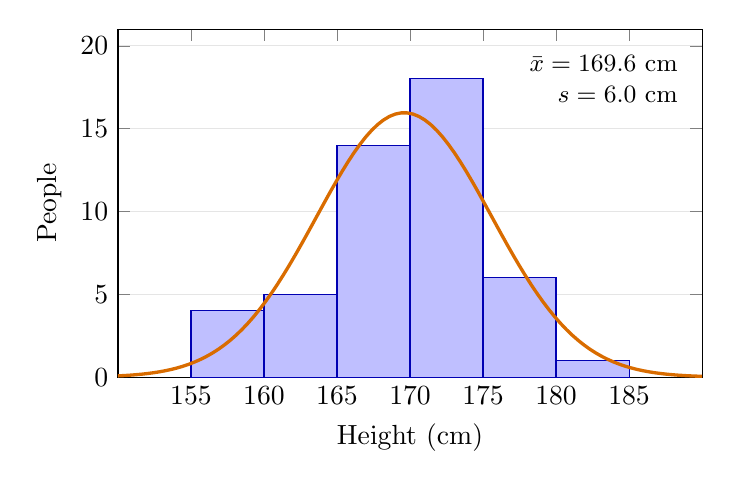
\begin{tikzpicture}
  \begin{axis}[
    width=9cm, height=6cm, ymin=0, ymax=21, xmin=150, xmax=190,
    xlabel={Height (cm)}, ylabel={People}, xtick={155,160,...,185},
    ymajorgrids, grid style={gray!20},
  ]
    \addplot[hist={bins=6, data min=155, data max=185}, fill=blue!25, draw=blue!70!black] table[row sep=\\, y index=0] {
      168\\ 174\\ 168\\ 168\\ 163\\ 169\\ 178\\ 173\\ 177\\ 172\\ 173\\ 171\\ 158\\ 176\\ 174\\ 173\\
      158\\ 158\\ 164\\ 167\\ 172\\ 170\\ 174\\ 166\\ 172\\ 173\\ 165\\ 182\\ 174\\ 178\\ 166\\ 165\\
      168\\ 169\\ 174\\ 172\\ 167\\ 163\\ 166\\ 179\\ 164\\ 172\\ 173\\ 160\\ 170\\ 179\\ 156\\ 168\\
    };
    % Mean 169.6 cm and standard deviation 6.0 cm; 48 people times the 5 cm bin width turns the density into counts.
    \addplot[very thick, orange!85!black, domain=150:190, samples=100] {48*5*exp(-(x - 169.6)^2/(2*6.0^2))/(6.0*sqrt(2*pi))};
    \node[anchor=north east, font=\small, align=right] at (axis cs:189,20) {$\bar x = 169.6$ cm\\$s = 6.0$ cm};
  \end{axis}
\end{tikzpicture}
